
% Default to the notebook output style

    


% Inherit from the specified cell style.




    
\documentclass[11pt]{article}

    
    
    \usepackage[T1]{fontenc}
    % Nicer default font (+ math font) than Computer Modern for most use cases
    \usepackage{mathpazo}

    % Basic figure setup, for now with no caption control since it's done
    % automatically by Pandoc (which extracts ![](path) syntax from Markdown).
    \usepackage{graphicx}
    % We will generate all images so they have a width \maxwidth. This means
    % that they will get their normal width if they fit onto the page, but
    % are scaled down if they would overflow the margins.
    \makeatletter
    \def\maxwidth{\ifdim\Gin@nat@width>\linewidth\linewidth
    \else\Gin@nat@width\fi}
    \makeatother
    \let\Oldincludegraphics\includegraphics
    % Set max figure width to be 80% of text width, for now hardcoded.
    \renewcommand{\includegraphics}[1]{\Oldincludegraphics[width=.8\maxwidth]{#1}}
    % Ensure that by default, figures have no caption (until we provide a
    % proper Figure object with a Caption API and a way to capture that
    % in the conversion process - todo).
    \usepackage{caption}
    \DeclareCaptionLabelFormat{nolabel}{}
    \captionsetup{labelformat=nolabel}

    \usepackage{adjustbox} % Used to constrain images to a maximum size 
    \usepackage{xcolor} % Allow colors to be defined
    \usepackage{enumerate} % Needed for markdown enumerations to work
    \usepackage{geometry} % Used to adjust the document margins
    \usepackage{amsmath} % Equations
    \usepackage{amssymb} % Equations
    \usepackage{textcomp} % defines textquotesingle
    % Hack from http://tex.stackexchange.com/a/47451/13684:
    \AtBeginDocument{%
        \def\PYZsq{\textquotesingle}% Upright quotes in Pygmentized code
    }
    \usepackage{upquote} % Upright quotes for verbatim code
    \usepackage{eurosym} % defines \euro
    \usepackage[mathletters]{ucs} % Extended unicode (utf-8) support
    \usepackage[utf8x]{inputenc} % Allow utf-8 characters in the tex document
    \usepackage{fancyvrb} % verbatim replacement that allows latex
    \usepackage{grffile} % extends the file name processing of package graphics 
                         % to support a larger range 
    % The hyperref package gives us a pdf with properly built
    % internal navigation ('pdf bookmarks' for the table of contents,
    % internal cross-reference links, web links for URLs, etc.)
    \usepackage{hyperref}
    \usepackage{longtable} % longtable support required by pandoc >1.10
    \usepackage{booktabs}  % table support for pandoc > 1.12.2
    \usepackage[inline]{enumitem} % IRkernel/repr support (it uses the enumerate* environment)
    \usepackage[normalem]{ulem} % ulem is needed to support strikethroughs (\sout)
                                % normalem makes italics be italics, not underlines
    

    
    
    % Colors for the hyperref package
    \definecolor{urlcolor}{rgb}{0,.145,.698}
    \definecolor{linkcolor}{rgb}{.71,0.21,0.01}
    \definecolor{citecolor}{rgb}{.12,.54,.11}

    % ANSI colors
    \definecolor{ansi-black}{HTML}{3E424D}
    \definecolor{ansi-black-intense}{HTML}{282C36}
    \definecolor{ansi-red}{HTML}{E75C58}
    \definecolor{ansi-red-intense}{HTML}{B22B31}
    \definecolor{ansi-green}{HTML}{00A250}
    \definecolor{ansi-green-intense}{HTML}{007427}
    \definecolor{ansi-yellow}{HTML}{DDB62B}
    \definecolor{ansi-yellow-intense}{HTML}{B27D12}
    \definecolor{ansi-blue}{HTML}{208FFB}
    \definecolor{ansi-blue-intense}{HTML}{0065CA}
    \definecolor{ansi-magenta}{HTML}{D160C4}
    \definecolor{ansi-magenta-intense}{HTML}{A03196}
    \definecolor{ansi-cyan}{HTML}{60C6C8}
    \definecolor{ansi-cyan-intense}{HTML}{258F8F}
    \definecolor{ansi-white}{HTML}{C5C1B4}
    \definecolor{ansi-white-intense}{HTML}{A1A6B2}

    % commands and environments needed by pandoc snippets
    % extracted from the output of `pandoc -s`
    \providecommand{\tightlist}{%
      \setlength{\itemsep}{0pt}\setlength{\parskip}{0pt}}
    \DefineVerbatimEnvironment{Highlighting}{Verbatim}{commandchars=\\\{\}}
    % Add ',fontsize=\small' for more characters per line
    \newenvironment{Shaded}{}{}
    \newcommand{\KeywordTok}[1]{\textcolor[rgb]{0.00,0.44,0.13}{\textbf{{#1}}}}
    \newcommand{\DataTypeTok}[1]{\textcolor[rgb]{0.56,0.13,0.00}{{#1}}}
    \newcommand{\DecValTok}[1]{\textcolor[rgb]{0.25,0.63,0.44}{{#1}}}
    \newcommand{\BaseNTok}[1]{\textcolor[rgb]{0.25,0.63,0.44}{{#1}}}
    \newcommand{\FloatTok}[1]{\textcolor[rgb]{0.25,0.63,0.44}{{#1}}}
    \newcommand{\CharTok}[1]{\textcolor[rgb]{0.25,0.44,0.63}{{#1}}}
    \newcommand{\StringTok}[1]{\textcolor[rgb]{0.25,0.44,0.63}{{#1}}}
    \newcommand{\CommentTok}[1]{\textcolor[rgb]{0.38,0.63,0.69}{\textit{{#1}}}}
    \newcommand{\OtherTok}[1]{\textcolor[rgb]{0.00,0.44,0.13}{{#1}}}
    \newcommand{\AlertTok}[1]{\textcolor[rgb]{1.00,0.00,0.00}{\textbf{{#1}}}}
    \newcommand{\FunctionTok}[1]{\textcolor[rgb]{0.02,0.16,0.49}{{#1}}}
    \newcommand{\RegionMarkerTok}[1]{{#1}}
    \newcommand{\ErrorTok}[1]{\textcolor[rgb]{1.00,0.00,0.00}{\textbf{{#1}}}}
    \newcommand{\NormalTok}[1]{{#1}}
    
    % Additional commands for more recent versions of Pandoc
    \newcommand{\ConstantTok}[1]{\textcolor[rgb]{0.53,0.00,0.00}{{#1}}}
    \newcommand{\SpecialCharTok}[1]{\textcolor[rgb]{0.25,0.44,0.63}{{#1}}}
    \newcommand{\VerbatimStringTok}[1]{\textcolor[rgb]{0.25,0.44,0.63}{{#1}}}
    \newcommand{\SpecialStringTok}[1]{\textcolor[rgb]{0.73,0.40,0.53}{{#1}}}
    \newcommand{\ImportTok}[1]{{#1}}
    \newcommand{\DocumentationTok}[1]{\textcolor[rgb]{0.73,0.13,0.13}{\textit{{#1}}}}
    \newcommand{\AnnotationTok}[1]{\textcolor[rgb]{0.38,0.63,0.69}{\textbf{\textit{{#1}}}}}
    \newcommand{\CommentVarTok}[1]{\textcolor[rgb]{0.38,0.63,0.69}{\textbf{\textit{{#1}}}}}
    \newcommand{\VariableTok}[1]{\textcolor[rgb]{0.10,0.09,0.49}{{#1}}}
    \newcommand{\ControlFlowTok}[1]{\textcolor[rgb]{0.00,0.44,0.13}{\textbf{{#1}}}}
    \newcommand{\OperatorTok}[1]{\textcolor[rgb]{0.40,0.40,0.40}{{#1}}}
    \newcommand{\BuiltInTok}[1]{{#1}}
    \newcommand{\ExtensionTok}[1]{{#1}}
    \newcommand{\PreprocessorTok}[1]{\textcolor[rgb]{0.74,0.48,0.00}{{#1}}}
    \newcommand{\AttributeTok}[1]{\textcolor[rgb]{0.49,0.56,0.16}{{#1}}}
    \newcommand{\InformationTok}[1]{\textcolor[rgb]{0.38,0.63,0.69}{\textbf{\textit{{#1}}}}}
    \newcommand{\WarningTok}[1]{\textcolor[rgb]{0.38,0.63,0.69}{\textbf{\textit{{#1}}}}}
    
    
    % Define a nice break command that doesn't care if a line doesn't already
    % exist.
    \def\br{\hspace*{\fill} \\* }
    % Math Jax compatability definitions
    \def\gt{>}
    \def\lt{<}
    % Document parameters
    \title{Behaavioural\_clonning\_report}
    
    
    

    % Pygments definitions
    
\makeatletter
\def\PY@reset{\let\PY@it=\relax \let\PY@bf=\relax%
    \let\PY@ul=\relax \let\PY@tc=\relax%
    \let\PY@bc=\relax \let\PY@ff=\relax}
\def\PY@tok#1{\csname PY@tok@#1\endcsname}
\def\PY@toks#1+{\ifx\relax#1\empty\else%
    \PY@tok{#1}\expandafter\PY@toks\fi}
\def\PY@do#1{\PY@bc{\PY@tc{\PY@ul{%
    \PY@it{\PY@bf{\PY@ff{#1}}}}}}}
\def\PY#1#2{\PY@reset\PY@toks#1+\relax+\PY@do{#2}}

\expandafter\def\csname PY@tok@mb\endcsname{\def\PY@tc##1{\textcolor[rgb]{0.40,0.40,0.40}{##1}}}
\expandafter\def\csname PY@tok@c1\endcsname{\let\PY@it=\textit\def\PY@tc##1{\textcolor[rgb]{0.25,0.50,0.50}{##1}}}
\expandafter\def\csname PY@tok@ne\endcsname{\let\PY@bf=\textbf\def\PY@tc##1{\textcolor[rgb]{0.82,0.25,0.23}{##1}}}
\expandafter\def\csname PY@tok@s2\endcsname{\def\PY@tc##1{\textcolor[rgb]{0.73,0.13,0.13}{##1}}}
\expandafter\def\csname PY@tok@vc\endcsname{\def\PY@tc##1{\textcolor[rgb]{0.10,0.09,0.49}{##1}}}
\expandafter\def\csname PY@tok@vi\endcsname{\def\PY@tc##1{\textcolor[rgb]{0.10,0.09,0.49}{##1}}}
\expandafter\def\csname PY@tok@s1\endcsname{\def\PY@tc##1{\textcolor[rgb]{0.73,0.13,0.13}{##1}}}
\expandafter\def\csname PY@tok@gt\endcsname{\def\PY@tc##1{\textcolor[rgb]{0.00,0.27,0.87}{##1}}}
\expandafter\def\csname PY@tok@nv\endcsname{\def\PY@tc##1{\textcolor[rgb]{0.10,0.09,0.49}{##1}}}
\expandafter\def\csname PY@tok@sr\endcsname{\def\PY@tc##1{\textcolor[rgb]{0.73,0.40,0.53}{##1}}}
\expandafter\def\csname PY@tok@s\endcsname{\def\PY@tc##1{\textcolor[rgb]{0.73,0.13,0.13}{##1}}}
\expandafter\def\csname PY@tok@kn\endcsname{\let\PY@bf=\textbf\def\PY@tc##1{\textcolor[rgb]{0.00,0.50,0.00}{##1}}}
\expandafter\def\csname PY@tok@sa\endcsname{\def\PY@tc##1{\textcolor[rgb]{0.73,0.13,0.13}{##1}}}
\expandafter\def\csname PY@tok@il\endcsname{\def\PY@tc##1{\textcolor[rgb]{0.40,0.40,0.40}{##1}}}
\expandafter\def\csname PY@tok@nf\endcsname{\def\PY@tc##1{\textcolor[rgb]{0.00,0.00,1.00}{##1}}}
\expandafter\def\csname PY@tok@mi\endcsname{\def\PY@tc##1{\textcolor[rgb]{0.40,0.40,0.40}{##1}}}
\expandafter\def\csname PY@tok@no\endcsname{\def\PY@tc##1{\textcolor[rgb]{0.53,0.00,0.00}{##1}}}
\expandafter\def\csname PY@tok@ge\endcsname{\let\PY@it=\textit}
\expandafter\def\csname PY@tok@mf\endcsname{\def\PY@tc##1{\textcolor[rgb]{0.40,0.40,0.40}{##1}}}
\expandafter\def\csname PY@tok@ow\endcsname{\let\PY@bf=\textbf\def\PY@tc##1{\textcolor[rgb]{0.67,0.13,1.00}{##1}}}
\expandafter\def\csname PY@tok@ni\endcsname{\let\PY@bf=\textbf\def\PY@tc##1{\textcolor[rgb]{0.60,0.60,0.60}{##1}}}
\expandafter\def\csname PY@tok@err\endcsname{\def\PY@bc##1{\setlength{\fboxsep}{0pt}\fcolorbox[rgb]{1.00,0.00,0.00}{1,1,1}{\strut ##1}}}
\expandafter\def\csname PY@tok@vg\endcsname{\def\PY@tc##1{\textcolor[rgb]{0.10,0.09,0.49}{##1}}}
\expandafter\def\csname PY@tok@cs\endcsname{\let\PY@it=\textit\def\PY@tc##1{\textcolor[rgb]{0.25,0.50,0.50}{##1}}}
\expandafter\def\csname PY@tok@nl\endcsname{\def\PY@tc##1{\textcolor[rgb]{0.63,0.63,0.00}{##1}}}
\expandafter\def\csname PY@tok@si\endcsname{\let\PY@bf=\textbf\def\PY@tc##1{\textcolor[rgb]{0.73,0.40,0.53}{##1}}}
\expandafter\def\csname PY@tok@kd\endcsname{\let\PY@bf=\textbf\def\PY@tc##1{\textcolor[rgb]{0.00,0.50,0.00}{##1}}}
\expandafter\def\csname PY@tok@gs\endcsname{\let\PY@bf=\textbf}
\expandafter\def\csname PY@tok@cp\endcsname{\def\PY@tc##1{\textcolor[rgb]{0.74,0.48,0.00}{##1}}}
\expandafter\def\csname PY@tok@fm\endcsname{\def\PY@tc##1{\textcolor[rgb]{0.00,0.00,1.00}{##1}}}
\expandafter\def\csname PY@tok@w\endcsname{\def\PY@tc##1{\textcolor[rgb]{0.73,0.73,0.73}{##1}}}
\expandafter\def\csname PY@tok@gi\endcsname{\def\PY@tc##1{\textcolor[rgb]{0.00,0.63,0.00}{##1}}}
\expandafter\def\csname PY@tok@ss\endcsname{\def\PY@tc##1{\textcolor[rgb]{0.10,0.09,0.49}{##1}}}
\expandafter\def\csname PY@tok@nn\endcsname{\let\PY@bf=\textbf\def\PY@tc##1{\textcolor[rgb]{0.00,0.00,1.00}{##1}}}
\expandafter\def\csname PY@tok@gp\endcsname{\let\PY@bf=\textbf\def\PY@tc##1{\textcolor[rgb]{0.00,0.00,0.50}{##1}}}
\expandafter\def\csname PY@tok@sh\endcsname{\def\PY@tc##1{\textcolor[rgb]{0.73,0.13,0.13}{##1}}}
\expandafter\def\csname PY@tok@ch\endcsname{\let\PY@it=\textit\def\PY@tc##1{\textcolor[rgb]{0.25,0.50,0.50}{##1}}}
\expandafter\def\csname PY@tok@sx\endcsname{\def\PY@tc##1{\textcolor[rgb]{0.00,0.50,0.00}{##1}}}
\expandafter\def\csname PY@tok@kt\endcsname{\def\PY@tc##1{\textcolor[rgb]{0.69,0.00,0.25}{##1}}}
\expandafter\def\csname PY@tok@k\endcsname{\let\PY@bf=\textbf\def\PY@tc##1{\textcolor[rgb]{0.00,0.50,0.00}{##1}}}
\expandafter\def\csname PY@tok@vm\endcsname{\def\PY@tc##1{\textcolor[rgb]{0.10,0.09,0.49}{##1}}}
\expandafter\def\csname PY@tok@m\endcsname{\def\PY@tc##1{\textcolor[rgb]{0.40,0.40,0.40}{##1}}}
\expandafter\def\csname PY@tok@gu\endcsname{\let\PY@bf=\textbf\def\PY@tc##1{\textcolor[rgb]{0.50,0.00,0.50}{##1}}}
\expandafter\def\csname PY@tok@gd\endcsname{\def\PY@tc##1{\textcolor[rgb]{0.63,0.00,0.00}{##1}}}
\expandafter\def\csname PY@tok@o\endcsname{\def\PY@tc##1{\textcolor[rgb]{0.40,0.40,0.40}{##1}}}
\expandafter\def\csname PY@tok@nb\endcsname{\def\PY@tc##1{\textcolor[rgb]{0.00,0.50,0.00}{##1}}}
\expandafter\def\csname PY@tok@cpf\endcsname{\let\PY@it=\textit\def\PY@tc##1{\textcolor[rgb]{0.25,0.50,0.50}{##1}}}
\expandafter\def\csname PY@tok@kr\endcsname{\let\PY@bf=\textbf\def\PY@tc##1{\textcolor[rgb]{0.00,0.50,0.00}{##1}}}
\expandafter\def\csname PY@tok@gr\endcsname{\def\PY@tc##1{\textcolor[rgb]{1.00,0.00,0.00}{##1}}}
\expandafter\def\csname PY@tok@nc\endcsname{\let\PY@bf=\textbf\def\PY@tc##1{\textcolor[rgb]{0.00,0.00,1.00}{##1}}}
\expandafter\def\csname PY@tok@gh\endcsname{\let\PY@bf=\textbf\def\PY@tc##1{\textcolor[rgb]{0.00,0.00,0.50}{##1}}}
\expandafter\def\csname PY@tok@sc\endcsname{\def\PY@tc##1{\textcolor[rgb]{0.73,0.13,0.13}{##1}}}
\expandafter\def\csname PY@tok@nt\endcsname{\let\PY@bf=\textbf\def\PY@tc##1{\textcolor[rgb]{0.00,0.50,0.00}{##1}}}
\expandafter\def\csname PY@tok@sb\endcsname{\def\PY@tc##1{\textcolor[rgb]{0.73,0.13,0.13}{##1}}}
\expandafter\def\csname PY@tok@cm\endcsname{\let\PY@it=\textit\def\PY@tc##1{\textcolor[rgb]{0.25,0.50,0.50}{##1}}}
\expandafter\def\csname PY@tok@se\endcsname{\let\PY@bf=\textbf\def\PY@tc##1{\textcolor[rgb]{0.73,0.40,0.13}{##1}}}
\expandafter\def\csname PY@tok@nd\endcsname{\def\PY@tc##1{\textcolor[rgb]{0.67,0.13,1.00}{##1}}}
\expandafter\def\csname PY@tok@kp\endcsname{\def\PY@tc##1{\textcolor[rgb]{0.00,0.50,0.00}{##1}}}
\expandafter\def\csname PY@tok@kc\endcsname{\let\PY@bf=\textbf\def\PY@tc##1{\textcolor[rgb]{0.00,0.50,0.00}{##1}}}
\expandafter\def\csname PY@tok@na\endcsname{\def\PY@tc##1{\textcolor[rgb]{0.49,0.56,0.16}{##1}}}
\expandafter\def\csname PY@tok@dl\endcsname{\def\PY@tc##1{\textcolor[rgb]{0.73,0.13,0.13}{##1}}}
\expandafter\def\csname PY@tok@c\endcsname{\let\PY@it=\textit\def\PY@tc##1{\textcolor[rgb]{0.25,0.50,0.50}{##1}}}
\expandafter\def\csname PY@tok@mo\endcsname{\def\PY@tc##1{\textcolor[rgb]{0.40,0.40,0.40}{##1}}}
\expandafter\def\csname PY@tok@go\endcsname{\def\PY@tc##1{\textcolor[rgb]{0.53,0.53,0.53}{##1}}}
\expandafter\def\csname PY@tok@sd\endcsname{\let\PY@it=\textit\def\PY@tc##1{\textcolor[rgb]{0.73,0.13,0.13}{##1}}}
\expandafter\def\csname PY@tok@mh\endcsname{\def\PY@tc##1{\textcolor[rgb]{0.40,0.40,0.40}{##1}}}
\expandafter\def\csname PY@tok@bp\endcsname{\def\PY@tc##1{\textcolor[rgb]{0.00,0.50,0.00}{##1}}}

\def\PYZbs{\char`\\}
\def\PYZus{\char`\_}
\def\PYZob{\char`\{}
\def\PYZcb{\char`\}}
\def\PYZca{\char`\^}
\def\PYZam{\char`\&}
\def\PYZlt{\char`\<}
\def\PYZgt{\char`\>}
\def\PYZsh{\char`\#}
\def\PYZpc{\char`\%}
\def\PYZdl{\char`\$}
\def\PYZhy{\char`\-}
\def\PYZsq{\char`\'}
\def\PYZdq{\char`\"}
\def\PYZti{\char`\~}
% for compatibility with earlier versions
\def\PYZat{@}
\def\PYZlb{[}
\def\PYZrb{]}
\makeatother


    % Exact colors from NB
    \definecolor{incolor}{rgb}{0.0, 0.0, 0.5}
    \definecolor{outcolor}{rgb}{0.545, 0.0, 0.0}



    
    % Prevent overflowing lines due to hard-to-break entities
    \sloppy 
    % Setup hyperref package
    \hypersetup{
      breaklinks=true,  % so long urls are correctly broken across lines
      colorlinks=true,
      urlcolor=urlcolor,
      linkcolor=linkcolor,
      citecolor=citecolor,
      }
    % Slightly bigger margins than the latex defaults
    
    \geometry{verbose,tmargin=1in,bmargin=1in,lmargin=1in,rmargin=1in}
    
    

    \begin{document}
    
    
    \maketitle
    
    

    
    \hypertarget{behavioral-cloning}{%
\section{\texorpdfstring{\textbf{Behavioral
Cloning}}{Behavioral Cloning}}\label{behavioral-cloning}}

\begin{center}\rule{0.5\linewidth}{\linethickness}\end{center}

\textbf{Behavioral Cloning Project}

The goals / steps of this project are the following: * Use the simulator
to collect data of good driving behavior * Build, a convolution neural
network in Keras that predicts steering angles from images * Train and
validate the model with a training and validation set * Test that the
model successfully drives around track one without leaving the road *
Summarize the results with a written report

\hypertarget{rubric-points}{%
\subsection{Rubric Points}\label{rubric-points}}

\hypertarget{here-i-will-consider-the-rubric-points-individually-and-describe-how-i-addressed-each-point-in-my-implementation.}{%
\subsubsection{\texorpdfstring{Here I will consider the
\href{https://review.udacity.com/\#!/rubrics/432/view}{rubric points}
individually and describe how I addressed each point in my
implementation.}{Here I will consider the rubric points individually and describe how I addressed each point in my implementation.}}\label{here-i-will-consider-the-rubric-points-individually-and-describe-how-i-addressed-each-point-in-my-implementation.}}

\begin{center}\rule{0.5\linewidth}{\linethickness}\end{center}

\hypertarget{files-submitted-code-quality}{%
\subsubsection{Files Submitted \& Code
Quality}\label{files-submitted-code-quality}}

\hypertarget{submission-includes-all-required-files-and-can-be-used-to-run-the-simulator-in-autonomous-mode}{%
\paragraph{1. Submission includes all required files and can be used to
run the simulator in autonomous
mode}\label{submission-includes-all-required-files-and-can-be-used-to-run-the-simulator-in-autonomous-mode}}

My project includes the following files: * clone.py containing the
script to create and train the model * drive.py for driving the car in
autonomous mode * Nvidia\_20e\_512\_022angleOffset folder *
Nvidia\_20e\_512\_022angleOffset.h5 containing a trained convolution
neural network * Nvidia\_20e\_512\_022angleOffset\_screen.mp4 containing
a screen recorded video of a full lap on track. *
Nvidia\_20e\_512\_022angleOffset\_video.mp4 containing the output of
video.py for the aboce full lap. * writeup\_behavioural\_clonning.md
summarizing the results

\hypertarget{submission-includes-functional-code}{%
\paragraph{2. Submission includes functional
code}\label{submission-includes-functional-code}}

Using the Udacity provided simulator and my drive.py file, the car can
be driven autonomously around the track by executing

\begin{Shaded}
\begin{Highlighting}[]
\ExtensionTok{python}\NormalTok{ drive.py Nvidia_20e_512_022angleOffset.h5}
\end{Highlighting}
\end{Shaded}

\hypertarget{submission-code-is-usable-and-readable}{%
\paragraph{3. Submission code is usable and
readable}\label{submission-code-is-usable-and-readable}}

The clone.py file contains the code for training and saving the
convolution neural network. The file shows the pipeline I used for
training and validating the model, and it contains comments to explain
how the code works.

\hypertarget{model-architecture-and-training-strategy}{%
\subsubsection{Model Architecture and Training
Strategy}\label{model-architecture-and-training-strategy}}

\hypertarget{an-appropriate-model-architecture-has-been-employed}{%
\paragraph{1. An appropriate model architecture has been
employed}\label{an-appropriate-model-architecture-has-been-employed}}

This model uses the NVIDIA convolutional neural Network (CNN)
architecture for learning which can be refered
\href{https://images.nvidia.com/content/tegra/automotive/images/2016/solutions/pdf/end-to-end-dl-using-px.pdf}{here}.
It is also modified to match the requirements.

The model includes ELU layers to introduce nonlinearity, and the data is
normalized in the model using a Keras lambda layer (code line 18).

\hypertarget{attempts-to-reduce-overfitting-in-the-model}{%
\paragraph{2. Attempts to reduce overfitting in the
model}\label{attempts-to-reduce-overfitting-in-the-model}}

The model contains 2 dropout layers in order to reduce overfitting
(clone.py lines 141).

The model was trained and validated on different data sets to ensure
that the model was not overfitting. The model was tested by running it
through the simulator and ensuring that the vehicle could stay on the
track.

\hypertarget{model-parameter-tuning}{%
\paragraph{3. Model parameter tuning}\label{model-parameter-tuning}}

The model used an adam optimizer, so the learning rate was manually set
to 0.001 (clone.py line 157).

\hypertarget{appropriate-training-data}{%
\paragraph{4. Appropriate training
data}\label{appropriate-training-data}}

Training data was chosen to keep the vehicle driving on the road. I have
used the sample data provided by Udacity, in addition to it there is 1
recorded lap in the forward direction of track 1, 1 recorded lap in the
reverse direction of track 1, and specific curve driving recordings in
both directions.

\hypertarget{model-architecture-and-training-strategy-1}{%
\subsubsection{Model Architecture and Training
Strategy}\label{model-architecture-and-training-strategy-1}}

\hypertarget{solution-design-approach}{%
\paragraph{1. Solution Design Approach}\label{solution-design-approach}}

The overall strategy for deriving a model architecture was to test
different models which are well known like LeNet (which is discussed
during the lectures), NVIDIA, VGG and several others.

I have tried the model LeNet. It is good for the straight lines and very
slight curves, When it came to sharp curves , it failed to predict the
correct angle.

Then for the next step I have tried NVIDIA model architecture. I
splitted my dataset into training set (80\%) and validation set (20\%).
But it has high MSE on validation set and low MSE in training set. this
is an example of Overfitting. FOr fixing this the model has been
modified by adding dropout layes. First dropout layer is after the
flatten layer and then the second one is after fully connected layer.

I tried running car in simulator. But still there are few spots where
car fell off the track. To improve the driving behaviour One final step
is taken into account. THe last convolution layer was removed. It just
on trial and error basis. ANd that made the trick.

At the end of the process, the vehicle is able to drive autonomously
around the track without leaving the road.

\hypertarget{final-model-architecture}{%
\paragraph{2. Final Model Architecture}\label{final-model-architecture}}

The final model architecture (clone.py lines 127-151) consisted of a
convolution neural network with the following layers and layer sizes
\ldots{} \textbar{}Layer (type) \textbar{} Output Shape \textbar{} Param
\# \textbar{} Connected to\textbar{}
\textbar{}-------------\textbar{}--------------\textbar{}---------\textbar{}-------------\textbar{}
\textbar{}image\_normalization (Lambda)\textbar{}(None, 64, 64,
3)\textbar{}0\textbar{}lambda\_input\_1{[}0{]}{[}0{]}\textbar{}
\textbar{}convolution\_1 (Convolution2D)\textbar{}(None, 30, 30,
24)\textbar{}1824\textbar{}image\_normalization{[}0{]}{[}0{]}\textbar{}
\textbar{}elu\_1 (ELU)\textbar{}(None, 30, 30,
24)\textbar{}0\textbar{}convolution\_1{[}0{]}{[}0{]}\textbar{}
\textbar{}convolution\_2 (Convolution2D)\textbar{}(None, 13, 13,
36)\textbar{}21636\textbar{}elu\_1{[}0{]}{[}0{]}\textbar{}
\textbar{}elu\_2 (ELU)\textbar{}(None, 13, 13,
36)\textbar{}0\textbar{}convolution\_2{[}0{]}{[}0{]}\textbar{}
\textbar{}convolution\_3 (Convolution2D)\textbar{}(None, 5, 5,
48)\textbar{}43248\textbar{}elu\_2{[}0{]}{[}0{]}\textbar{}
\textbar{}elu\_3 (ELU)\textbar{}(None, 5, 5,
48)\textbar{}0\textbar{}convolution\_3{[}0{]}{[}0{]}\textbar{}
\textbar{}convolution\_4 (Convolution2D)\textbar{}(None, 3, 3,
64)\textbar{}27712\textbar{}elu\_3{[}0{]}{[}0{]}\textbar{}
\textbar{}elu\_4 (ELU)\textbar{}(None, 3, 3,
64)\textbar{}0\textbar{}convolution\_4{[}0{]}{[}0{]}\textbar{}
\textbar{}flatten\_1 (Flatten)\textbar{}(None,
576)\textbar{}0\textbar{}elu\_4{[}0{]}{[}0{]}\textbar{}
\textbar{}dropout\_1 (Dropout)\textbar{}(None,
576)\textbar{}0\textbar{}flatten\_1{[}0{]}{[}0{]}\textbar{}
\textbar{}hidden1 (Dense)\textbar{}(None,
100)\textbar{}57700\textbar{}dropout\_1{[}0{]}{[}0{]}\textbar{}
\textbar{}elu\_5 (ELU)\textbar{}(None,
100)\textbar{}0\textbar{}hidden1{[}0{]}{[}0{]}\textbar{}
\textbar{}dropout\_2 (Dropout)\textbar{}(None,
100)\textbar{}0\textbar{}elu\_5{[}0{]}{[}0{]}\textbar{}
\textbar{}hidden2 (Dense)\textbar{}(None,
50)\textbar{}5050\textbar{}dropout\_2{[}0{]}{[}0{]}\textbar{}
\textbar{}elu\_6 (ELU)\textbar{}(None,
50)\textbar{}0\textbar{}hidden2{[}0{]}{[}0{]}\textbar{}
\textbar{}hidden3 (Dense)\textbar{}(None,
10)\textbar{}510\textbar{}elu\_6{[}0{]}{[}0{]}\textbar{}
\textbar{}elu\_7 (ELU)\textbar{}(None,
10)\textbar{}0\textbar{}hidden3{[}0{]}{[}0{]}\textbar{}
\textbar{}steering\_angle (Dense)\textbar{}(None,
1)\textbar{}11\textbar{}elu\_7{[}0{]}{[}0{]}\textbar{}

\hypertarget{creation-of-the-training-set-training-process}{%
\paragraph{3. Creation of the Training Set \& Training
Process}\label{creation-of-the-training-set-training-process}}

To capture good driving behavior, I first recorded one lap on track one
using center lane driving. Here is an example image of center lane
driving:

\begin{figure}
\centering
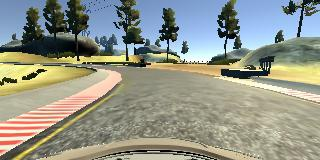
\includegraphics{./examples/forward.jpg}
\caption{alt text}
\end{figure}

I then recorded the vehicle recovering from the left side and right
sides of the road back to center so that the vehicle would learn to
\ldots{}. These images show what a recovery looks like starting from
\ldots{} :

\begin{figure}
\centering
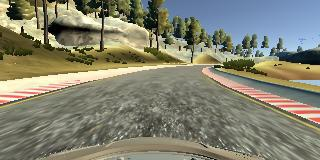
\includegraphics{./examples/reverse.jpg}
\caption{alt text}
\end{figure}

I then recorded three laps on track one in the reverse direction to
further generalize the dataset.

To augment the data sat, I also flipped images and angles thinking that
this would give wider range of the data to train the model. Which will
also help in reducing overfitting.

left and right camera images are also used to train the model. Right
camera image with an offset of -0.22 in the steering angle, and the left
camera image with an offset of 0.22 in the steering angle.

After the collection process, there are 46,000 data points. I have
preprocessed this data by cropping 40 pixels from top of the images
which have unusable and unnecessary details, and 20 pixels from the
buttom to remove the vehicle hood. Now these images are resized to
64x64.

I finally randomly shuffled the data set and put 20\% of the data into a
validation set.

I used this training data for training the model. The validation set
helped determine if the model was over or under fitting. The ideal
number of epochs was 20 as evidenced by me.


    % Add a bibliography block to the postdoc
    
    
    
    \end{document}
